\subsection{Generación de rayos X}

Los rayos X se producen cuando un haz de electrones de alta energía, acelerados a través de un voltaje que supera los miles de voltios, chocan con un material. Dichos electrones interaccionan con los electrones orbitales o los núcleos del material por varios mecanismos diferentes que dan lugar a emisiones energéticas. El dispositivo experimental más habitual para la generación de rayos X se conoce como "tubo de rayos X", donde los electrones son acelerados gracias a una diferencia de potencial desde el cátodo hasta el ánodo, y siendo el ánodo el material que genera los rayos X.

Existen dos mecanismos fundamentales para la generación de rayos X: la radiación característica y la radiación de frenado o bremsstrahlung. 

La radiación característica se produce cuando un electrón proyectil ioniza los átomos del ánodo, es decir, arranca un electrón interno del átomo. Esto hace que el electrón de la capa K que ha sido arrancado deje un hueco, situación que es muy inestable para el átomo, lo que conlleva a que un electrón de las capas externas ocupe ese nivel vacío. Este proceso va acompañado por la emisión de un fotón de rayos X característicos del material con que se ha hecho el ánodo y cuya energía es igual a la diferencia de energías de los órbitales electrónicos tal como se aprecia en la figura (\ref{figure_radiacion_cobre}).

\begin{figure}[t]
	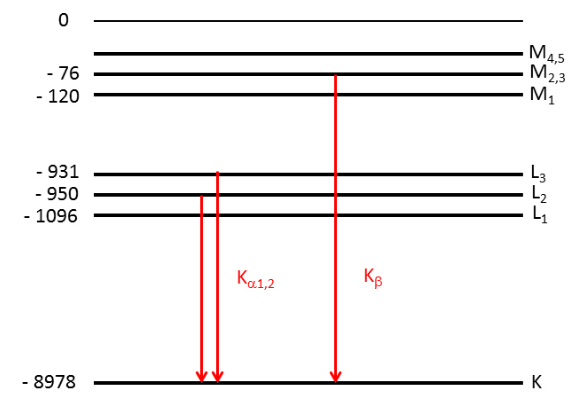
\includegraphics[width=\linewidth]{radiacion_caracteristica_cobre}
	\caption{Diagrama de niveles energéticos de rayos X para el cobre (en eV). En líneas rojas se muestran las transiciones más probables $K_{\alpha}$ y $K_{\beta}$}
	\label{figure_radiacion_cobre}
\end{figure}

La radiación de frenado se produce cuando un electrón proyectil se frena y/o desvía por interacciones electrostáticas al pasar lo suficientemente cerca de los núcleos del ánodo, perdiendo energía cinética que es emitida en forma de fotón de rayos X. El electrón puede perder cualquier cantidad de energía cinética, lo cual conlleva a un continuo de valores en la energía de los fotones, al contrario que la radiación característica. Sin embargo, dicha energía de los fotones nunca podrá ser superior a la energía inicial de los electrones proyectiles, pues deben satisfacer igualmente la ecuación de la energía

\begin{equation}
	E = h \sigma = \frac{hc}{\lambda} = eV \label{eq_energia}
\end{equation}

Donde $h$ es la constante de Planck, $\sigma$ es la frecuencia del electrón (o la radiación), $c$ es la velocidad de la luz, $\lambda$ la longitud de onda, $e$ la carga del electrón y $V$ el potencial.

\subsection{Ley de Bragg}

En 1913, William Henry Bragg y su hijo William Lawrence Bragg publican la que conocemos hoy día como la Ley de Bragg, una relación que permite predecir los ángulos en los que los rayos X son difractados por un material con estructura atómica periódica (materiales cristalinos). La interferencia es constructiva cuando la diferencia de fase entre la radiación emitida por diferentes átomos es proporcional a $2\pi$, condición que se expresa según la ecuación

\begin{equation}
	n \lambda = 2d sin(\theta) \label{eq_bragg}
\end{equation}

Siendo $n$ un número entero, $\lambda$ la longitud de onda de los rayos X, $d$ la distancia entre planos de la red cristalina y $\theta$ el ángulo entre los rayos incidentes y los planos de dispersión. En la figura (\ref{figure_ley_bragg}) podemos ver una representación gráfica del fenómeno

\begin{figure}[t]
	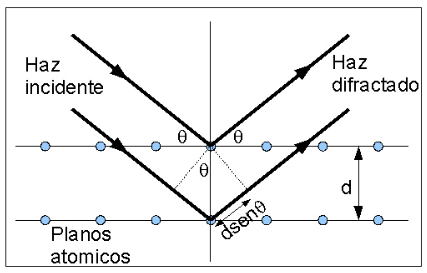
\includegraphics[width=\linewidth]{ley_bragg}
	\caption{Esquema de difracción de rayos X en un cristal}
	\label{figure_ley_bragg}
\end{figure}

Combinando las ecuaciones \eqref{eq_energia} y \eqref{eq_bragg} podemos expresar la distancia interplanar tal que

\begin{equation}
	d = \frac{hcn}{2Esin(\theta)} \label{eq_distancia}
\end{equation}

Podemos relacionar la Ley de Bragg con la radiación de frenado mediante lo que se conoce como "ángulo mínimo", que es aquel ángulo para el cual se empieza a observar radiación de frenado. Dado que el borde inferior del espectro de la radiación de frenado determina una energía máxima de la radiación X, podemos establecer la relación

\begin{equation}
	sin(\theta_{min}) = \frac{hc}{2deV} \label{eq_angulo_min}
\end{equation}

Donde se ha hecho $E = eV$ según la ecuación \eqref{eq_energia}.

\subsection{Materiales. Estructura del LiF y KBr}

Tanto el fluoruro de litio como el bromuro de potasio son cristales con estructura cúbica centrada en las caras, por lo que tienen ocho elementos por célula. Sus densidades son $2.64 g/cm^3$ y $2.74 g/cm^3$ y tienen un parámetro de red $a$ de valor $4.02$ y $6.61$ ángstroms, respectivamente.

\begin{equation}
	a = (\frac{4m}{N_{A}\rho})^{1/3} \label{eq_parametro_red}
\end{equation}

Siendo $N_A$ el número de Avogadro, $m$ la masa molar del material y $\rho$ su densidad. El factor 4 en el numerador hace referencia a que de los 8 elementos por celda, la mitad son átomos distintos.

Conocida la distancia interplanar y el parámetro de red para estos materiales podemos conocer los índices de Miller $(h,k,l)$ de la esructura cristalina mediante

\begin{equation}
	d_{hkl}^{2} = \frac{a^2}{h^2 + k^2 + l^2} \label{eq_miller}
\end{equation}